\begin{ZhChapter}

\chapter{Proposed Algorithm}
This section will provide a brief overview of this chapter: First we will introduce the architecture of our algorithm and use a simple flowchart to provide a basic introduction to the proposed algorithm. Next we want to provide an in-depth explanation of our proposed algorithm, including the underlying concepts and the rationale behind our approach. Lastly we will provide a detailed description of our software and hardware specifications, as well as the setup procedures.
\section{The Architecture of Algorithm} %Chapter 3.1
\begin{figure*}[htbp]
    \centering
    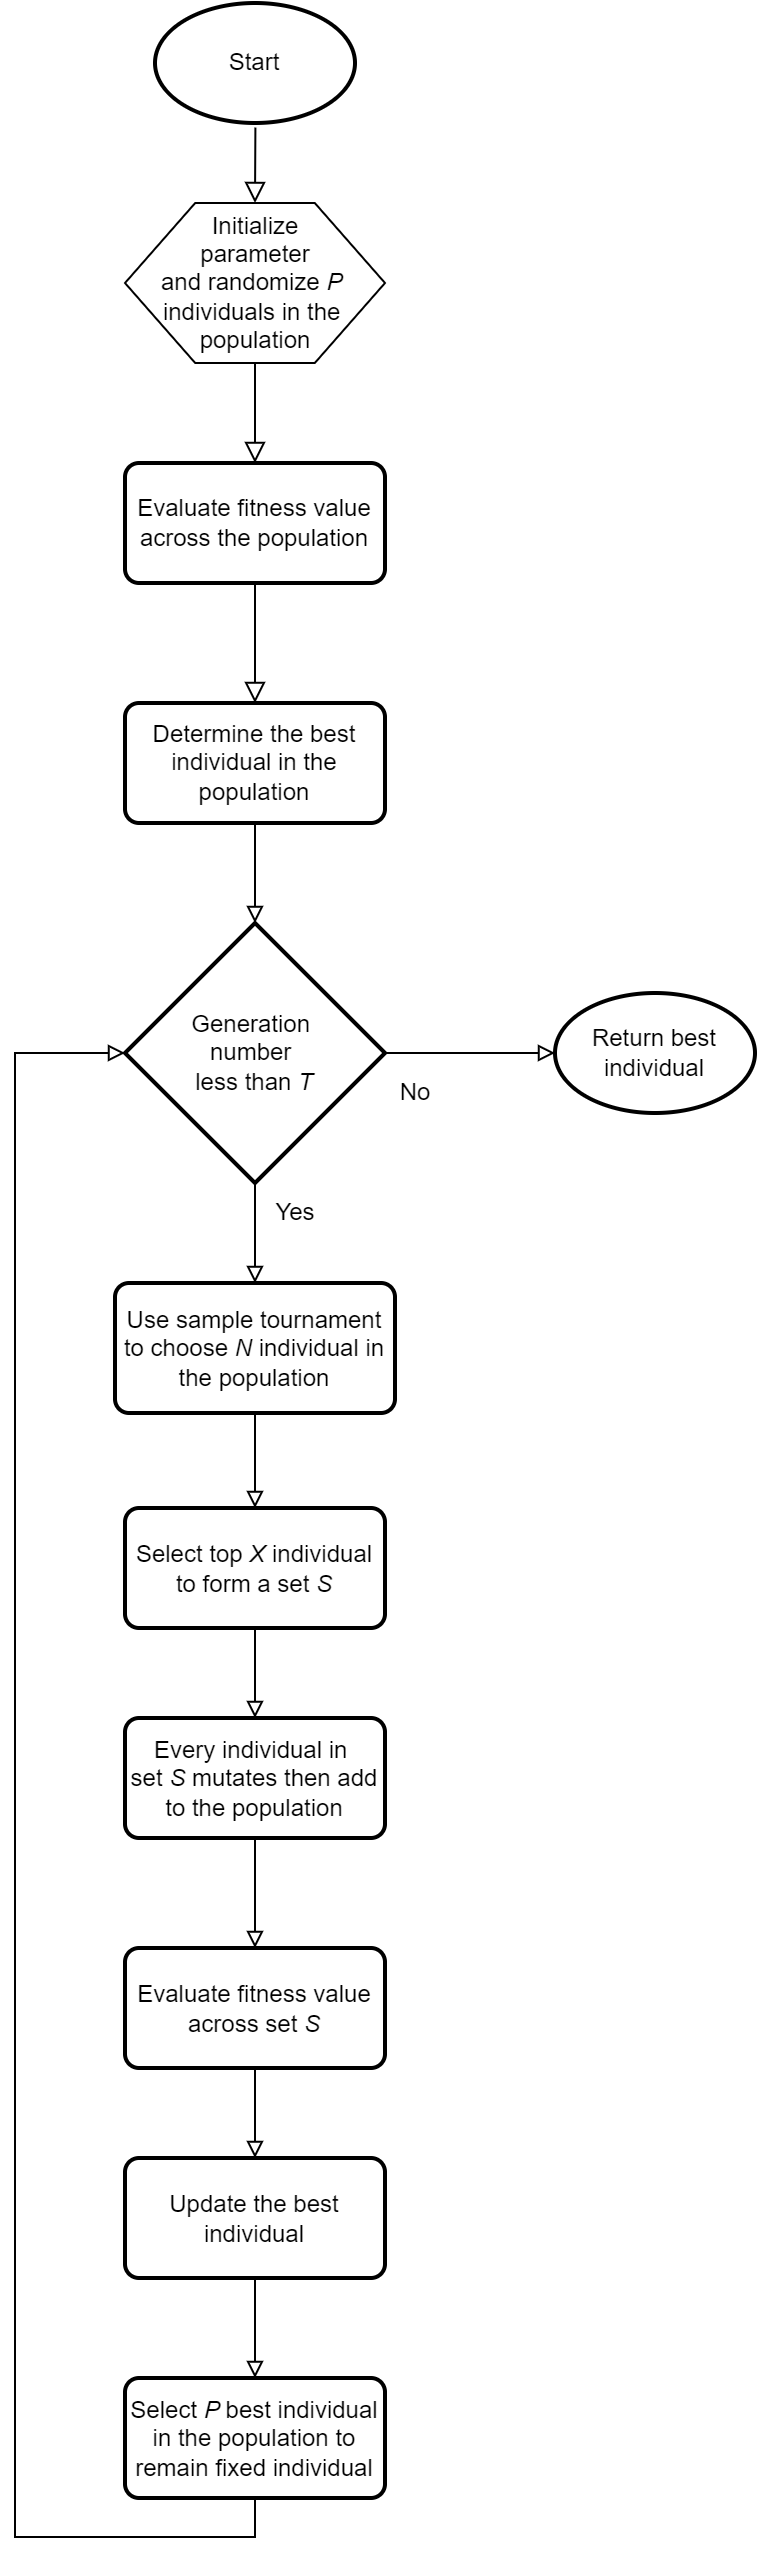
\includegraphics[width = 1\textwidth]{image/FlowChart.png}
    \caption{FlowChart for Efficiency-based GP}
    \label{fig: FlowChart}
\end{figure*}
% \section{Experimental Environment Setup}

% \subsection{Software Setup}
% In our software setup, we run our code in Ubuntu 24.04. The Python version we employ is 3.8, and the Pytorch version is X. Within Python and Pytorch, we utilize the following packages: Some package.

% \subsection{Hardware Setup}
% In our hardware setup, we run our code on an AMD Ryzen 5 5600X 6-Core Processor. The system is equipped with 32GB of memory, operating at a frequency of DDR4-3600MHz. Additionally, we utilize an NVIDIA GeForce RTX 3060 Ti GPU for our computational needs.

\section{Main Method}
% \documentclass{article}

\begin{algorithm}
    \caption{Efficiency-based GP to generate loss function}\label{alg:cap}
    \begin{algorithmic}
        \State Initialize:$P = \space $x, $T =\space $x, $N = \space $x, $M_{ST} = \space0.5$
        \State Randomly initialize population which include P trees
        \State Evaluate GP fitness function $F$ for each individual in the population
        \State Determine the best individual
        \While{generation number < $T$}
        \State Sample tournament G $\sim$ Uniform (P)
        \State Select top $N$ trees from $G$ to form a set $S$
        \For{Individual in $S$}
        \If {$rand_1 < M_{ST}$}
        \State Apply subtree mutation to the generated child
        \Else
        \State Apply one-point mutation to the individual
        \EndIf
        \If {Functional\_check() is true}
        \State add individual to population
        \EndIf
        \EndFor
        \State Evaluated GP fitness function $F$ for each generated child individual
        \State Update the best individual
        \State Select $P$ best trees from population to form a new population containing $P$ trees
        \EndWhile
    \end{algorithmic}
\end{algorithm}

\section{Implementation Details}

\subsection{Requirements}

\begin{table*}[htbp]
\centering
\caption{Software requirements} \label{tab: softwareSpec}
\makebox[\linewidth][c]{
    \renewcommand\arraystretch{1.2}{
        \begin{tabular}{| l | c  c  c  c |}
        \hline
        Package Type & Software Name & Version & Remark & License \\
        \hline
        Operating System & Ubuntu &  24.04 & N/A & N/A \\
        Programming Language & Python & 3.11 & N/A & N/A\\
        Programming Language & Pytorch & N/A & N/A & N/A\\
        \hline
        \end {tabular}
    }}
\end {table*}
Table \ref{tab: softwareSpec} shows our software requirements. We run our code in Ubuntu 24.04. The Python version we employ is 3.8, and the Pytorch version is X. Within Python and Pytorch, we utilize the following packages: Some package.

\begin{table*}[htbp]
\centering
\caption{Hardware requirements} \label{tab: hardwareSpec}
\makebox[\linewidth][c]{
    \renewcommand\arraystretch{1.2}{
        \begin{tabular}{| l | c |}
        \hline
        Hardware Type & Name \\
        \hline
        CPU & AMD Ryzen 5 5600X 6-Core Processor \\
        Memory & DDR4-3600MHz 32 GB \\
        Graphic Card & NVIDIA GeForce RTX 3060 Ti \\
        \hline
        \end {tabular}
    }}
\end {table*}

Table \ref{tab: hardwareSpec} shows our hardware requirements. We run our code on an AMD Ryzen 5 5600X 6-Core Processor. The system is equipped with 32GB of memory, operating at a frequency of DDR4-3600MHz. Additionally, we utilize an NVIDIA GeForce RTX 3060 Ti GPU for our computational needs.
\subsection{Environment Setup}

\subsection{Implementation Steps}
% \subsection{}
% 定義定義定義定義定義定義\cite{latex2e},定義定義定義定義,定義定義定義定義定義定義定義定義定義定義,定義定義。

% \begin{table*}[htbp]
%     \centering
%     \caption{表格範例標題} \label{tab: complexity}
%     \makebox[\linewidth][c]{
%     \renewcommand\arraystretch{1.2}{
%         \begin{tabular}{| l | c  c  c  c |}
%         \hline
%         Protocol & $P$ & $CS_1$ & $CS_2$ & $RG$ \\
%         \hline
%         MSSMul & $O(1)$, $O(1)$, N/A & $O(n-t)$, $O(n)$, $O(1)$ & $O(n-t)$, $O(n)$, N/A & $O(1)$, $O(n)$, $O(n)$ \\
%         SC & $O(1)$, $O(1)$, N/A & $O(n-t)$, $O(n)$, $O(1)$ & $O(n-t)$, $O(n)$, N/A & $O(1)$, $O(n)$, $O(n)$ \\
%         \hline 
%         \end {tabular}
%     }}
% \end {table*}

% \section{模型說明(小標)}

% 說明說明說明說明,說明說明說明說明說明說明說明說明說明說明說明說明,說明說明說明說明說明說明說明說明。

% \begin{figure*}[htbp]
%     \centering
%     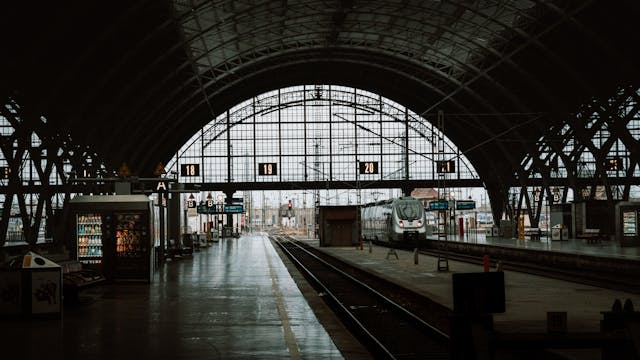
\includegraphics[width = 0.5\textwidth]{image.jpeg}
%     \caption{Cool train station}
%     \label{fig: image}
% \end{figure*}

\end{ZhChapter}